\documentclass{report} %[twoside] ?
\usepackage[utf8]{inputenc}
\usepackage[german]{babel}
\usepackage{graphicx}
\usepackage{array}
\usepackage{amssymb, mathtools}
\usepackage{setspace}
\usepackage{multirow}
\usepackage{subcaption}
\usepackage{caption}
\usepackage{changepage}
\usepackage{xurl}
\usepackage{titlesec}
\captionsetup{font=footnotesize}
\titleformat{\chapter}[display]
    {\normalfont\huge\bfseries}{\chaptertitlename\ \thechapter}{20pt}{\Huge}
\titlespacing*{\chapter}{0pt}{0pt}{40pt}

\title{
    Evaluation of Machine Learning Models for Leakage Detection in Water Distribution Networks
}

\author{Julian Hendrik Freiherr Bock von Wülfingen}
\date{19.06.2022}

\begin{document}

\onehalfspacing

\pagenumbering{gobble}

\begin{titlepage}

	\begin{center}

        \vspace*{\baselineskip}

        {\Large Universität Bielefeld}
        
        \vspace{1.75\baselineskip}

        {\LARGE \scshape Evaluation of Machine Learning \\ Models for Leakage Detection in \\ Water Distribution Networks\par} % Title

        \vspace{5\baselineskip}
        
        {\Large Julian Hendrik Freiherr Bock von Wülfingen}
        
        \vspace{2\baselineskip}

        {\Large Bachelorarbeit\vspace{1em}}
        
        \textit{im Studiengang Kognitive Informatik \vspace{1em} \\ AG Machine Learning}
	
        \vfill

        \vspace{0.3\baselineskip}
        
        Erstgutachter:	  André Artelt\\
        Zweitgutachter:	  Johannes Brinkrolf\\
        Abgabe:		    15.07.2022

    \end{center}

\end{titlepage}

\tableofcontents

\cleardoublepage
\pagenumbering{arabic}

\chapter{Einleitung}

Wasserverteilungssysteme (engl. Water Distribution Networks, WDNs) gehören zu den wichtigsten Infrastrukturen
 einer Gesellschaft, in welcher der Anspruch besteht, Trinkwasser in ausreichender Menge und Qualität auf die
 Haushalte zu verteilen. Da der Hauptteil dieser Netzwerke jedoch unter der Erde vergraben liegt, sind WDNs
 anfällig für plötzliche sowie schleichende Schäden, die häufig ohne direkt sichtbare Indikatoren
 auftreten können. Das Wasser kann sich hierbei verunreinigen und geht in Massen verloren. Weltweit beträgt
 der jährliche Wasserverlust, welcher vor allem durch solche Lecks vorangetrieben wird, 126 Milliarden
 Kubikmeter. Auch wenn es in Deutschland nur 5\% des gesamten Wasseraufkommens sind, kann es in manchen
 Extremfällen bis über 50\% gehen. Der finanzielle Schaden allein beträgt weltweit knapp 40 Milliarden USD
 jährlich todo. Doch nicht nur aus finanzieller Sicht ist dies dramatisch. In Zeiten des Klimawandels
 muss auf eine effiziente Nutzung endlicher Ressourcen Acht gegeben werden.

Das Erkennen von Lecks muss demnach schnell und akkurat sein. Alleine das Freilegen der Rohrleitungen kostet viel
 Zeit [Quelle], weswegen die Rate fälschlicher Erkennung niedrig gehalten werden sollte. Auch wenn manche Lecks
 einfach zu erkennen sind, beispielsweise durch sichtbar austretendes Wasser oder spürbaren Druckverlust, ist in
 den meisten Fällen der Wasserverlust unterirdisch. Um solche Arten zu erkennen, können Sensoren installiert
 werden, die den aktuellen Druck in den Rohren messen. Da das Installieren von Drucksensoren unter der Erde
 ebenso einen größeren Aufwand bedeuten, haben [Q1] und [Q2] eine Methode entwickelt, eine optimale
 Sensoren-Verteilung zu ermöglichen.

\section*{Inhalt der Arbeit}

Thema dieser Bachelorarbeit ist es, die Sensordaten zu analysieren und durch ein datengetriebenes Modell
 potentielle Lecks in WDNs frühzeitig zu erkennen. Hierfür ist die Arbeit in drei Kapitel aufgeteilt:
 Zuerst wird auf die theoretischen Grundlagen der Anomaliedetektion in WDNs sowie ausgewählter Modelle und
 Ideen des Maschinellen Lernens eingegangen.
In diesem Zuge wird auch untersucht, welche Metriken zur Evaluation von Detektions-Modellen geeignet sind.
Wie zuvor erwähnt, ist dies kein triviales Thema, da neben der Erkennungsrate auch auf eine niedrige
 Fehlalarm-Quote sowie eine kurze Zeit vom Auftreten der Lecks bis zu ihrem Erkennen geachtet werden muss.

Weiterführend wird auf die Methodik eingegangen. Hierfür wird zunächst der Datensatz analysiert gefolgt von
 der Implementation des Erkennungsmodells. Grundlage für ein solches Modell bilden sogenannte digitale Zwillinge,
 welche digitale Repräsentationen realer Abläufe sind; Die Sensorwerte werden simuliert und mit den echten
 Werten verglichen. Eine zu hohe Diskrepanz kann dann als Problemfall gemeldet werden. In der Vergangenheit
 wurden diese simulierte Netzwerke häufig als hydraulische Systeme gelöst, also einer Menge an spezifisch auf
 das WDN angepassten, mathematisch-physikalischen Gleichungen. Diese fordern jedoch in der Modellierung hohe
 Expertise und besitzen während der Kalibrierung eine starke Komplexität durch viele Freiheitsgrade. Somit
 werden häufiger Methoden aus dem Bereich des Maschinellen Lernens verwendet, welche die Gesetze der Hydraulik
 nicht kennen müssen und anhand großer, problem-spezifischer Datenmengen selbst lernen.

Zuletzt werden die Ergebnisse der Methoden vorgestellt und anschließend diskutiert. Hierbei wird auf die
 Probleme lokaler Optima sowie die Realisierbarkeit der Modelle eingegangen.


\chapter{Grundlagen}

\section{Maschinelles Lernen}

\subsection*{Eingrenzung}

Das umfassende Feld des Maschinellen Lernens (ML) lässt sich grob in zwei Arten unterteilen;
 Supervised und Unsupervised Learning. In beiden Fällen wird eine Funktion $f: X \rightarrow Y$ gelernt,
 jedoch besitzen die Trainingsdaten für Unsupervised ML keine Informationen für die zu prognostizierende
 Variable $y \in Y$. Dies kann beispielsweise interessant sein für eine Clustering-Aufgabe, in welcher der
 Datensatz in zwei oder mehrere Gruppen aufgeteilt werden soll und vorher nichts über diese Verteilung bekannt
 ist. Die Leck-Detektion benötigt jedoch weitere Informationen; Denn im Gegensatz zu Unsupervised ML ist beim
 Supervised ML diese sogenannte Ground Truth (GT) bekannt und das jeweilige Problem lässt sich anhand der
 Definition des Bildbereichs weiter eingrenzen: Die für die Arbeit wichtigen Arten sind hier die binäre
 Klassifikation und die Regression.

Bei der binären Klassifikation soll jeder Datenpunkt $x \in X$ einer von zwei Klassen $y \in \{0, 1\}$ zugewiesen
 werden. Auf unser Problem der Leck-Detektion angewendet, hieße eine Klassifikation eines Zeitpunkts in
 Klasse $1$, dass irgendwo in dem WDN ein Leck existiert, wohingegen Klasse $0$ die Abwesenheit sämtlicher
 Lecks impliziert. Für die Regression wird jedem Datenpunkt ein reeller Wert $y \in \mathbb{R}$ zugewiesen.
Wie dieses Konzept übernommen werden kann, ist in Kapitel ? weiter beschrieben. 


\subsection*{Modelle des Maschinellen Lernens}

Für jeden Anwendungsbereich gibt es eine Vielzahl an verschiedenen Algorithmen, welche eine gegebene Aufgabe
 lösen können. Die in dieser Arbeit benutzten Modelle werden im Folgenden erklärt. Hierbei ist wichtig, zwischen
 Parametern und Hyperparametern zu unterscheiden. Ersteres sind dabei die Variablen und Gewichte, die während
 des Lernprozesses optimiert oder gefunden werden. Die sogenannten Hyperparameter sind Einstellungen, welche
 vor dem Training konfiguriert werden und damit das Ergebnis erheblich verändern können.

\begin{itemize}

   \item \textbf{k-Nearest Neighbors (kNN)} ist ein einfaches Modell, bei dem ein neuer Datenpunkt nach der
    Mehrheit seiner Nachbarn $(x_i, y_i)$ in einem n-dimensionalen Koordinatensystem klassifiziert wird. Der
    Hyperparameter $k$ bestimmt hierbei, wie groß die zu betrachtende Nachbarschaft ist. Sei
            $\mathcal{N}(\hat{x}, \mathcal{D}, k)$
    die Menge der $k$ am nächsten zu $\hat{x}$ liegenden Punkte aus $\mathcal{D}$, dann ist
            $P(\hat{x}=c|\hat{x}, \mathcal{D}, k) = \frac{1}{k} |\{x_i | x_i \in \mathcal{N}(\hat{x}, \mathcal{D}, k), y_i=c\}|$
    der Anteil der Klasse $c$ in der Nachbarschaft. Die finale Klasse des neuen Datenpunktes $\hat{x}$ ist dann
    gegeben durch die am meisten vertretene Klasse:
    \begin{equation}
            f_{kNN}(\hat{x}) = \underset{c \in \{1..C\}}{\mathrm{argmax}}\ P(\hat{x}=c|\hat{x}, \mathcal{D}, k)
    \end{equation}
    Zusätzlich lässt sich mit dem Hyperparameter der Gewichtung einstellen, ob Punkte, die sich im Raum weiter
    weg befinden, weniger stark gewichtet werden.

   \item \textbf{Multi-Layer Perceptron (MLP)} versucht, ein künstliches neuronales Netz zu erschaffen, indem es
    mehrere Perzeptronen aneinanderreiht. Ein Perzeptronen steht hier für ein Neuron, welches mehrere Eingabewerte
    hat und daraus einen Ausgabewert erstellt. Dafür wird jeder Eingabewert mit einem speziell dafür gelernten
    Gewicht multipliziert und anschließend aufsummiert. Zu dieser Summe kann dann noch ein Schwellwert $\theta$
    hinzuaddiert werden, welches ebenso beim Lernen optimiert wird. Als letztes wird darauf eine sogenannte
    Aktivierungsfunktion angewendet, was dann die Ausgabe des Perzeptron bildet. Die Aktivierungsfunktionen,
    welche in dieser Arbeit betrachtet worden sind, sind die logistische Funktion, der Hyperbeltangens und der
    Rectified Linear Unit (ReLU):
    \begin{align}
        \text{logistic}(x) &= \frac{1}{1+e^{-x}}\\
        \text{tanh}(x)     &= 1-\frac{2}{e^{2x}+1}\\
        \text{relu}(x)     &= \max(0, x)
    \end{align}
    Die Ausgabe eines Perzeptrons ist also
    \begin{equation}
            f(x) = f_{activation}(\sum_i(w_ix_i)+\theta),
    \end{equation}
    wobei $f_{activation}$ die Aktivierungsfunktion und $w$ die gelernten Gewichte sind. Ein MLP ist dann eine
    Ansammlung vieler einzelner Perzeptronen in möglicherweise mehreren Schichten. Dafür besteht eine Schichte
    aus mehreren, in parallel arbeitenden Perzeptronen, deren Eingabe die Ausgabe aus der vorherigen Schicht
    darstellt. Ihre Ausgabe ist dann wieder Eingabe der folgenden Schicht. Abbildung ? zeigt so eine Struktur.
    Dabei ist die Anzahl der Schichten sowie die Menge an Perzeptronen pro Schicht ein Hyperparameter.

    Die einzelnen Gewichte lernen kann dieses Modell indem es die Datenpunkt durch das (untrainierte) Netz
    schickt und die Vorhersage mit der GT vergleicht. In einem Verfahren, was sich Backtracking nennt, werden
    im Grunde die Gewichte, welcher zu einer falschen Entscheidung führten geschwächt, während Gewichte, die
    eine richtige Entscheidung herbeiführen konnten, verstärkt werden. Diese Technik lässt sich durch weitere
    Hyperparameter, welche zum Beispiel die Rate der Verstärkung beeinflussen, optimieren.

   \item \textbf{Linear Regression (LR)} ist eine Regressionsmethode, die versucht, eine Gerade im
    n-dimensionalen Raum zu schaffen, welche die Abstände zu den bekannten Datenpunkten minimiert. Der
    Wert eines neuen Datenpunktes wird nun durch die parametrische Funktion
    \begin{equation}
        f(\hat{x}) = \sum_i w_ix_i - \theta
    \end{equation}
    prognostiziert. Um die optimalen Gewichte zu finden, nutzt LR den Mean
    Squared Error (MSE), welcher gegeben ist als
    \begin{equation}
        MSE = \frac{1}{n} \sum_i(y_i-f(x_i))^2
    \end{equation}
    und die durchschnittliche, quadrierte Abweichung der Punkte von der Linie beschreibt. Die finalen
    Gewichte sind nun $w = \text{argmin}_{\tilde{w}} MSE$.

   \item \textbf{Ridge (L2)} und \textbf{Lasso (L1)} Regression sind Erweiterungen der LR indem sie einen
    Regularisierungsterm zum MSE hinzufügen, welcher Einfluss auf die optimalen Gewichte hat. Für L2 werden
    die einzelnen Gewichte quadriert und mit einem Hyperparameter $\alpha$\footnote{In der Literatur auch
    häufig $\lambda$ genannt.} multipliziert. Die optimalen Gewichte werden
    damit berechnet: 
    \begin{equation}
        w = \text{argmin}_{\tilde{w}} MSE + \alpha||\tilde{w}||_2^2.
    \end{equation}
    Dadurch werden zu hohe Gewichte und damit Overfitting, was in Kapitel ? weiter erklärt wird, bestraft.
    L1 nutzt die absoluten Werte der Gewichte:
    \begin{equation}
        w = \text{argmin}_{\tilde{w}} MSE + \alpha||\tilde{w}||_1.
    \end{equation}
    Während L2 aufgrund der Natur quadratischer Funktionen den Wert von $\alpha$ nur asymptotisch gegen $0$ gehen
    lassen kann, kann L1 diesen komplett auf $0$ setzen. Damit kann einfacher mit Dimensionen umgegangen werden,
    die nur wenig Einfluss auf das Endergebnis haben.

\end{itemize}

Das korrekte Setzen der Hyperparameter gehört zu dem Fachbereich des Fine Tunings von Modellen und kann
 gravierende Effekte auf das Endergebnis haben. Methoden um diese Aufgabe anzugehen, werden in den
 nächsten Kapiteln beschrieben.


\section{Evaluation und Metriken}

Um einschätzen zu können, wie gut ein Modell mit gegebenen Hyperparametern und ausgewählten Daten das Problem
 löst, wird eine Metrik benötigt. Eine solche ist definiert als Funktion, welche die wahren und die
 prognostizierten Werte annimmt und einen einzigen Wert\footnote{typischerweise zwischen 0 und 1} als
 Indikator, wie gut in einer gewissen Disziplin abgeschnitten wurde, zurückgibt. Die meisten Metriken,
 die in dieser Arbeit verwendet werden, können aus der Konfusionsmatrix berechnet werden. Für ein binäres
 Klassifikationsproblem hat sie den folgenden Aufbau:

\begin{center}
    \hspace{3.1cm}Echtes Label \\ Modell Ausgabe
    \begin{tabular}{ c | c c | }
      & 1 & 0 \\ 
     \hline
     1 & TP & FP \\  
     0 & FN & TN \\
     \hline  
    \end{tabular}
\end{center}

Auf der Diagonalen steht TP (True Positive) für die Menge an positiven Fällen, die auch als solche erkannt
 wurden, und TN (True Negative) für alle negative Fälle, die ebenfalls richtig vom Modell erkannt wurden.
 Die anderen Werte stehen für keine Übereinstimmung der Werte; FN (False Negative) steht für fälschlicherweise
 als negativ klassifizierte Datenpunkte und FP (False Positive) für welche, an denen das Modell ohne Grund
 positiv angeschlagen hat. Tabelle ? zeigt ausgewählte Metriken, die in dieser Arbeit benutzt werden und was sie
 in diesem Kontext bedeuten.

 \renewcommand{\arraystretch}{2}
\begin{tabular}{ m{6em} m{7em} m{16em} }
    Metrik & Berechnung & Bedeutung \\
    \hline
    Accuracy              & $\frac{TP+TN}{TP+TN+FP+FN}$ & Wie oft lag der Algorithmus richtig? \\
    Recall (Sensitivität) & $\frac{TP}{TP+FN}$          & Wie gut wurden echte Lecks erkannt? \\
    Specificity           & $\frac{TN}{TN+FP}$          & Wie gut wurde 'alles ok' erkannt? \\
    Precision             & $\frac{TP}{TP+FP}$          & Wie viele erkannte Lecks waren auch wirklich Lecks? \\
    Detection Time        & Mittelwert vom Auftreten eines Lecks bis zur Erkennung & Wie viele Zeiteinheiten dauerte es bis zum Erkennen?
\end{tabular}

Hierbei ist wichtig anzumerken, dass auch wenn die Accuracy alle Werte der Konfusionsmatrix in die Bewertung
 mit einfließen lässt, diese nur als grobe Einschätzung genutzt werden sollte, da sie im Vergleich zu den anderen
 Metriken keine Begründung liefert, wie die anderen Metriken. Zudem kann sie auf unbalancierten Datensätzen ein
 falsches Bild vermitteln\footnote{TODO bsp. 99\%}.

Um die Metriken erheben zu können, muss man jedoch definieren, welche Datenpunkte hierfür genutzt werden
 und welche nicht. Das nächste Kapitel gibt Aufschluss darüber, wie dies bewerkstelligt werden kann.


\section{Hyperparameter Tuning}

Das Ergebnis eines Machine Learning Modells hängt stark von den gewählten Hyperparametern ab. Diese zu
 optimieren gehört zu den Kernaufgaben im Lebenszyklus des Modellierungsprozesses, für die jedoch eine
 Verlässliche Aussage der Metriken wichtig ist. Man sollte davon absehen, auf den gleichen Daten zu testen,
 auf denen man bereits trainiert hat. Dabei kann es nämlich unbemerkt zu Overfitting kommen, was bedeutet,
 dass das Modell nicht genug generalisiert, sondern die Eigenheiten des Datensatzes, wie zum Beispiel Rauschen,
 lernt. Dadurch funktioniert es schlechter auf nicht gesehenen Daten. Weiter sind Metriken nicht mehr so
 aussagekräftig, wenn nur bereits Bekanntes abgefragt wird\footnote{Mit $k=1$ hätte kNN einen Fehler von $0$, falls
 auf den gleichen Daten getestet und trainiert wird.}. Die Test- und Trainingsdaten sollten also disjunkt sein.

\subsection*{Train-Test-Split}

Beim Train-Test-Split wird die Datenmenge in zwei Gruppen aufgeteilt: Das Train-Set und das Test-Set.
 Typischerweise beträgt die größe des Test-Sets zwischen 20\% und 33\% der gesamten Daten. Da bei diesem Split
 auf neuen Daten getestet wird, zwingt es einen dazu, das Modell so zu gestalten, dass es gut generalisieren
 kann. Bei einer unglücklichen Wahl des Test-Sets, kann es jedoch immer noch passieren, dass die Metriken
 einen falschen Eindruck hinterlassen\footnote{TODO 33\% class1 in train, 0 in test}.

\subsection*{Cross-Validation}

Die Lösung dieses Problems ist das wiederholte Anwenden eines Train-Test-Splits. Bei der sogenannten
 k-Fold Cross-Validation wird der Datensatz in k gleich große Mengen unterteilt. Mit dieser Aufteilung
 wird dann k-Mal der Prozess des Trainierens und Testens gestartet, wobei jedes mal ein anderes der k Sets als
 Test-Set gewählt wird. Abbildung ? visualisiert dieses Vorgehen. Die Ergebnisse der k Durchläufe werden
 anschließend gemittelt und zeigen damit eine weitaus robustere Einschätzung der Güte auf. Das k liegt hier
 typischerweise zwischen 5 und 10\footnote{Es gibt einen Spezialfall, indem k gleich der größe des Datensatzes
 ist. Eine solche Einstellung nennt sich Leave-One-Out Cross-Validation, bei welcher immer auf allen Datenpunkten
 mit Ausnahme eines einzigen Punktes trainiert wird. Dies ist jedoch nicht Thema dieser Arbeit.}.

\subsection*{Grid-Search}

Mit dieser Technik können nun verlässlich die Hyperparameter analysiert werden. Mit der Methode des Exhaustive
 Grid-Search lassen sich alle Hyperparameter testen, indem das kartesisches Produkt der möglichen Einstellungen
 gebildet und auf allen Kombinationen mittels Cross-Validation trainiert und getestet wird. So wird für kNN einmal
 mit uniformer Gewichtung der Nachbarn jede Einstellung für k getestet und einmal mit Distanz-bedingter Gewichtung.
 Das Ergebnis zeigt nun die optimale Einstellung für die Gewichtsfunktion und das k an. Ebenso können weitere
 Relationen ausgelesen werden; Beispielsweise könnte für ein höheres k die Distanz-bedingte Gewichtung besser
 funktionieren, für kleinere k jedoch eher die uniforme Gewichtung.


\section{Anomaliedetektion}

Für die Detektion von Lecks in WDNs gibt es mehrere Ansätze, welche sich in aktive und passive
 Strategien einteilen lassen.

\begin{itemize}
    
    \item Die \textbf{aktiven Verfahren}, auch Hardware-basierte Verfahren, sind Strategien, die mittels
     spezialisierter Technik aktiv nach Brüchen in den Rohren suchen. Hierfür könnten zum Beispiel
     Schallgeneratoren oder Kameras benutzt werden. Dabei steht jeder Suchvorgang in der Regel für sich
     und bildet keinen Verlauf ab. Zudem sind aktive Verfahren sowohl Zeit- als auch Ressourcenintensiv.

    \item Dahingegen sind \textbf{passive Verfahren}, oder auch Modell-basierte Verfahren, darauf ausgelegt
     ein kontinuierliches Bild über den aktuellen Zustand des Netzwerkes zu geben und bei Anomalien Alarm zu
     schlagen. Hierfür wird die bereits erwähnte Technik der digitalen Zwillinge angewendet, indem das reale
     Netz, welches durch eine Menge an Sensoren durchgehend überwacht wird, durch ein virtuell simuliertes
     Netzwerk erweitert wird. Mit der Annahme, dass die Simulation den Normalzustand, also eine Leckfreie
     Version des Netzwerkes, abbildet, können aus zu hohen Differenzen Anomalien abgeleitet werden. Die
     Simulation kann auf zwei Wege erstellt werden. Die Hydraulic Model Based Verfahren nutzen spezifisch
     kalibrierte, hydraulische Gleichungen. Sie berücksichtigen alles von der genauen Struktur und Höhenlage
     über Material bis hin zur Rohrdicke und Alter. Die resultierende Menge an Gleichungen ist daher sehr
     komplex und sensibel gegenüber Ungenauigkeit in der Beschreibung. Auf der anderen Seite stehen die
     Hydraulic Measurement Based (oder auch datengetriebenen) Verfahren. Diese nutzen maschinelles Lernen um
     mittels Langzeitdaten des Netzwerkes Vorhersagen zu treffen. Dadurch ist kein Vorwissen über die
     hydraulischen Eigenschaften des Netzwerkes nötig, da das notwendige Wissen von den Algorithmen gelernt wird.
    
\end{itemize}

In dieser Arbeit geht es um die datengetriebenen, also die passiven, auf vorangegangenen Messwerten
 basierten, Verfahren. Ein solches Modell funktioniert in zwei Schritten. Im ersten Schritt wird das
 digitale Netzwerk simuliert. Hierfür wird für jeden echten Sensor ein digitaler Sensor erstellt. Dieser
 schätzt den eigenen Druckwert anhand der aktuellen Druckwerte aller anderen Sensoren. Möglicherweise können
 auch direkt vorangegangene Messwerte in diese Vorhersage mit eingebaut werden. Wird dies für jeden Sensor
 gemacht, entsteht ein digitales Netzwerk, bei dem jeder digitale Sensor kein Wissen über seinen realen Wert
 hat. Im nächsten Schritt wird dann zuerst die Differenz der Netzwerke berechnet. Ist momentan kein Leck im
 WDN, so sollten diese Differenzen klein sein, während Lecks zu höheren Differenzen führen. Hier gilt es nun,
 einen Threshold zu finden, ab dem eine Differenz zu hoch ist, um im Normalbereich zu liegen. Ist dieser
 abhängig von dem jeweiligen Sensor, so stellt sich ebenso die Frage, bei wie vielen Sensoren eine Differenz
 als ‘zu hoch’ gelten muss, damit das gesamte Modell Alarm schlägt.

Wie in Kapitel ? schon angemerkt, unterscheidet sich die Güte eines Modells auch darin, welche Metrik
 benutzt wird. So folgt aus dem finanziellen und ökologischen Schaden eines Lecks, dass potentielle Lecks
 früh erkannt werden sollen; Eine niedrige Detection Time und hohe Sensitivität (bzw. Recall) ist gefordert.
 Während das eigentliche Reparieren eines Rohrs in relativ geringer Zeit absolviert werden kann, ist das, was
 drum herum getan werden muss, umso zeit- und ressourcenintensiver. Vom Absperren der Straße über das Schließen
 der Ventile bis hin zum Aufgraben des Bodens bis zum Rohr können viele Stunden vergehen [TODO Quelle]. Ebenso kann
 das Zugraben des Loches viel Zeit brauchen, da sich zum Beispiel manche aufgeschüttete Bodenschichten erst Zeit
 zum sich setzen benötigen, bevor weitergemacht werden kann. Eine hohe Rate an falschen Alarmierungen, also eine
 niedrige Präzision, sollte dementsprechend auch vermieden werden. Verknüpft mit anderen Detektionsverfahren,
 wie zum Beispiel der aktiven Suche zum Überprüfen potentieller Lecks, kann der Wert auf eine optimale Präzision
 jedoch auch wieder geschmälert werden\footnote{Da diese Verfahren jedoch wie besagt auch aufwändig sind, sollte
 dennoch auf die Präzision geachtet werden.}.



\chapter{Anomaliedetektion}

Für die Detektion von Lecks in WDNs gibt es mehrere Ansätze, welche sich in aktive und passive
 Strategien einteilen lassen \cite{lee2021development}.

\begin{itemize}
    
    \item Die \textbf{aktiven Verfahren}, auch hardwarebasierte Verfahren, sind Strategien, die mittels
     spezialisierter Technik aktiv nach Brüchen in den Rohren suchen. Hierfür könnten zum Beispiel
     Schallgeneratoren oder Kameras benutzt werden. Dabei steht jeder Suchvorgang in der Regel für sich
     und bildet keinen Verlauf ab. Zudem sind aktive Verfahren sowohl Zeit- als auch Ressourcenintensiv.

    \item Dahingegen sind \textbf{passive Verfahren}, oder auch modellbasierte Verfahren, darauf ausgelegt
     ein kontinuierliches Bild über den aktuellen Zustand des Netzwerkes zu geben und bei Anomalien Alarm zu
     schlagen. Hierfür wird die bereits erwähnte Technik der digitalen Zwillinge angewendet, indem das reale
     Netz, welches durch eine Menge an Sensoren durchgehend überwacht wird, durch ein virtuell simuliertes
     Netzwerk erweitert wird. Mit der Annahme, dass die Simulation den Normalzustand, also eine leckfreie
     Version des Netzwerkes, abbildet, können aus zu hohen Differenzen Anomalien abgeleitet werden. Die
     Simulation kann auf zwei Wege erstellt werden. Die Hydraulic Model Based Verfahren nutzen spezifisch
     kalibrierte, hydraulische Gleichungen. Sie berücksichtigen alles von der genauen Struktur und Höhenlage
     über Material bis hin zur Rohrdicke und Alter. Die resultierende Menge an Gleichungen ist daher sehr
     komplex und sensibel gegenüber Ungenauigkeit in der Beschreibung. Auf der anderen Seite stehen die
     Hydraulic Measurement Based (oder auch datengetriebenen) Verfahren. Diese nutzen maschinelles Lernen um
     mittels Langzeitdaten des Netzwerkes Vorhersagen zu treffen. Dadurch ist kein Vorwissen über die
     hydraulischen Eigenschaften des Netzwerkes nötig, da das notwendige Wissen von den Algorithmen gelernt wird.
    
\end{itemize}

In dieser Arbeit geht es um die datengetriebenen, also die passiven, auf vorangegangenen Messwerten
 basierten, Verfahren. Ein solches Modell funktioniert in zwei Schritten. Im ersten Schritt wird das
 virtuelle Netzwerk simuliert. Hierfür wird für jeden echten Sensor ein digitaler Sensor erstellt. Dieser
 schätzt den eigenen Druckwert anhand der aktuellen Druckwerte aller anderen Sensoren. Möglicherweise können
 auch direkt vorangegangene Messwerte in diese Vorhersage mit eingebaut werden. Wird dies für jeden Sensor
 gemacht, entsteht ein virtuelles Netzwerk, bei dem jeder digitale Sensor kein Wissen über seinen realen Wert
 hat. Im nächsten Schritt wird dann zuerst die Differenz der Netzwerke berechnet. Ist momentan kein Leck im
 WDN, so sollten diese Differenzen klein sein, während Lecks zu höheren Differenzen führen. Hier gilt es nun,
 einen Threshold zu finden, ab dem eine Differenz zu hoch ist, um im Normalbereich zu liegen. Ist dieser
 abhängig von dem jeweiligen Sensor, so stellt sich ebenso die Frage, bei wie vielen Sensoren eine Differenz
 als ‘zu hoch’ gelten muss, damit das gesamte Modell Alarm schlägt.

Wie in Kapitel \ref{Chapter-ML} schon angemerkt, unterscheidet sich die Güte eines Modells auch darin, welche Metrik
 benutzt wird. So folgt aus dem finanziellen und ökologischen Schaden eines Lecks, dass potentielle Lecks
 früh erkannt werden sollen; Eine niedrige Detection Time und hohe Sensitivität ist gefordert.
 Während das eigentliche Reparieren eines Rohrs in relativ geringer Zeit absolviert werden kann, ist das, was
 drum herum getan werden muss, umso zeit- und ressourcenintensiver. Vom Absperren der Straße über das Schließen
 der Ventile bis hin zum Aufgraben des Bodens bis zum Rohr können viele Stunden vergehen \cite{breakTime}. Ebenso
 kann das Zugraben des Loches viel Zeit brauchen, da sich zum Beispiel manche aufgeschüttete Bodenschichten erst
 Zeit zum sich setzen benötigen, bevor weitergemacht werden kann. Eine hohe Rate an falschen Alarmierungen, also
 eine niedrige Präzision, sollte dementsprechend auch vermieden werden. Verknüpft mit anderen Detektionsverfahren,
 wie zum Beispiel der aktiven Suche zum Überprüfen potentieller Lecks, kann der Wert auf eine optimale Präzision
 jedoch auch wieder geschmälert werden\footnote{Da diese Verfahren jedoch wie besagt auch aufwändig sind, sollte
 dennoch auf die Präzision geachtet werden.}.


\chapter{Modellierung \label{Chapter-Methods}}

Um die verschiedenen Modelle testen zu können, werden zwei Ansätze vorgestellt, welche jeweils auf zwei Datensätzen
 trainiert werden. Diese wurden dabei durch ein Simulations-Tool erzeugt, welches im Folgenden erklärt wird.

\section{Datensatz}

\subsection*{WNTR Simulation}

Grundlage für das Trainieren und Evaluieren der Modelle bilden Simulationen des Water Network Tool for Resilience
 (WNTR) \cite{klise2018overview} Auf Basis eines EPANET-Netzwerkes können durch die mannigfaltigen
 Umgebungsvariablen, welche Parameter, wie das zugrunde liegende Hydraulikmodell, aber auch Ereignisse, wie
 Rohrbrüche verschiedenster Stärken, einschließen, eine vielzahl an Szenarien erstellt werden. So besteht der erste
 Datensatz aus ad-hoc generierten, einfachen Szenarien, die durch ihre geringere Komplexität einen schnellen
 Evaluationszyklus gewähren. Hingegen besteht der zweite Datensatz aus vorgenerierten Szenarien, welche mit
 Unsicherheiten und weiter definierten Bedarf, weitaus realistischere Daten darstellen.
 Beide Datensätze nutzen das gleiche WDN als Basis:
 Das sogenannte EPANET Example Network 1 (auch als Net1 zu finden). Dessen Topologie ist in Abbildung
 \ref{fig:practice-wdn} gezeigt und besitzt als verhältnismäßig kleines Netzwerk neun Knotenpunkte, einen Tank
 und ein Reservoir.

\begin{figure}
    \centering
    \fbox{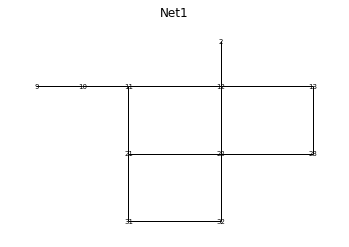
\includegraphics[width=0.7\textwidth]{res/practice-wdn}}
    \caption{Aufbau des Netzwerkes.}
    \label{fig:practice-wdn}
\end{figure}

\subsubsection*{Der ad-hoc Datensatz}

Die Ausgabe der WNTR-Simulation ist eine einfache Tabelle, in welcher für jeden Knoten stündlich die Werte des
 Wasserdrucks eingetragen sind. Abbildung \ref{fig:practice-sim} zeigt einen Beispielverlauf der Druckwerte im Normalzustand sowie
 in Leckszenarien verschiedener Stärken. Diese können mit der Funktion
 \begin{center}
    \texttt{add\_leak(network, area, start\_time, end\_time)},
 \end{center}
 wobei “area” als betroffene Größe in Metern die Stärke
 des Lecks kennzeichnet, zu einem Knoten hinzugefügt werden. Die finalen Einstellungen sehen eine zufällige Stärke
 im Bereich von 0.0009 bis 0.0014 vor. Betrachtet man die Werte der Knoten zu einem bestimmten Zeitpunkt am Tag,
 so sieht man, dass (nach einer bis zu zehntägigen Eingewöhnungsphase, welche im weiteren Verlauf herausgeschnitten
 wird) diese exakt gleich sind. Damit die Modelle nicht die genauen Werte lernen, wird ein geringes,
 normalverteiltes Rauschen hinzu addiert (siehe Abbildung \ref{fig:practice-noise}).

\begin{figure}[ht]
    \centering
    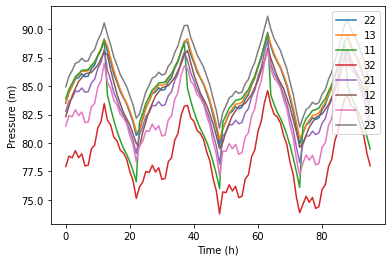
\includegraphics[width=0.45\textwidth]{res/practice-sim-noleak.png}
    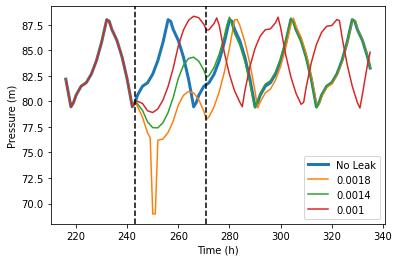
\includegraphics[width=0.45\textwidth]{res/practice-sim-leak.png}
    \caption{Beispielhafte Druckverläufe. Links ein leckfreies Szenario für eine Auswahl an Knoten. Rechts
        für den Knoten 12 ein Vergleich verschiedener Stärken des Lecks.}
    \label{fig:practice-sim}
\end{figure}

\begin{figure}[ht]
    \centering
    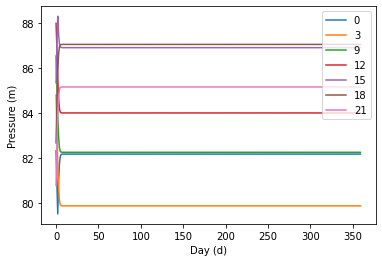
\includegraphics[width=0.44\textwidth]{res/practice-noise-days.png}
    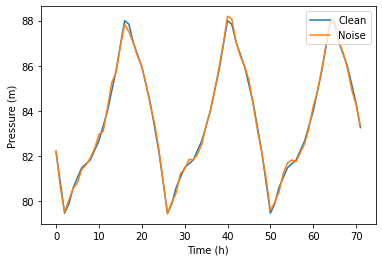
\includegraphics[width=0.44\textwidth]{res/practice-noise-applied.png}
    \caption{Beispielhafte Druckverläufe des Knotens 12. Links sind die Druckwerte ausgewählter Stunden über das
        Jahr angegeben. Nach der Eingewöhnungsphase sind ide vollständig konstant. Rechts ist der Einfluss des
        kleinen Rauschens gezeigt.}
    \label{fig:practice-noise}
\end{figure}

\subsubsection*{LeakDB}

Der realistischere Datensatz LeakDB \cite{vrachimis2018leakdb} ist eine Ansammlung von 1000 Szenarien, welche
 jeweils über ein Jahr andauern und eine doppelt so hohe, zeitliche Auflösung, also halbstündlich, haben.
 Betrachtet man hier ebenso den Verlauf des Wertes einer Tageszeit, so kann man, im Vergleich zum ad-hoc
 Datensatz, hier saisonale Ereignisse und die Unsicherheit direkt erkennen.

\subsection*{Datenformat}

Damit die Daten weiterhin als Zeitfolgen betrachtet werden können, gleichzeitig aber auf mehreren Szenarien
 trainieren und evaluieren werden kann, ist der Definitionsbereich des Modells nicht als $\mathbb{R}^{N \times d}$
 definiert, wobei $N$ die Anzahl an Datenpunkten und $d$ die Anzahl Sensoren ist, sondern als
 $\mathbb{R}^{N \times p \times d}$, mit $p$ als Datenpunkte pro Zeitfolge\footnote{Wichtig anzumerken ist hier,
 dass das $p$ kein fester Wert ist, sondern unterschiedlich für jede der $N$ Zeitfolgen sein kann.} und $N$
 als Anzahl Zeitfolgen. Damit kann dem Modell eine Liste an Zeitfolgen übergeben werden,
 dessen Rückgabewert aus $\{0, 1\}^{N \times p}$ ist, also jedem Zeitpunkt das Label 0 oder 1, für kein Leck
 oder Leck, gibt. Im Folgenden bezeichnet $\mathcal{X}$ diese Liste an Zeitfolgen,
 $X_i \in \mathcal{X}$ eine einzelne Zeitfolge und $x_{i, j} = (x_{i, j}^{(1)}, \dots, x_{i, j}^{(d)}) \in X_i$ den $j$-ten
 Zeitpunkt aus Zeitfolge $i$ mit $x_{i, j}^{(k)}$ als dessen $k$-ten Sensorwert.

Die Analyse für die Metriken, welche aus der
 Konfusionsmatrix berechnet werden, geschieht nun nicht auf den einzelnen Zeitpunkten $x_{i, j}$, sondern auf
 den Zeitfolgen $X_i$. Eine Zeitfolge gilt als Leck-Szenario mit Label 1, falls mindestens ein Zeitpunkt
 innerhalb des Szenarios als Leck gekennzeichnet wurde. Andernfalls bekommt die leckfreie Folge das Label 0.
 Mit diesen Werten kann nun die Konfusionsmatrix gebildet und die Metriken berechnet werden. Ein weiterer Vorteil
 der Betrachtung der Datenpunkte als Liste an Zeitfolgen ist die Berechnung der Detektionszeit: Diese kann nun
 innerhalb einer Zeitfolge als zeitliche Differenz des Auftretens eines Lecks bis hin zu seiner Erkennung gesehen
 werden, gegeben es existiert ein Leck, welches auch wirklich gefunden wurde. Die Menge an Differenzen kann dann
 hinsichtlich Mittelwert, Standardabweichung und Median untersucht werden.

Ein weiterer Schritt beim Vorbereiten der Daten ist das hinzufügen von Zeitinformationen. Während die aus der
 Simulation hervorgehenden Druckwerte nur mit Zeitschritt, also einer natürlichen Nummerierung, indiziert sind,
 ist für die weitere Bearbeitung der Werte eine weitere Informationen benötigt: Die Uhrzeit (im Quellcode auch
 \texttt{hour of the day}) wird durch das Anwenden von \texttt{modulo 24} auf den ursprünglichen
 Index\footnote{Aufgrund der doppelten, zeitlichen Auflösung muss für LeakDB dieser Index noch halbiert werden,
 bevor Modulo gerechnet werden kann.} berechnet und kann damit die Zeitliche Einordnung, welche aus der
 Datenanalyse als annähernd periodisch angesehen ist, erleichtern.


\section{Algorithmen}

Die im Rahmen dieser Arbeit bearbeiteten Strategien sind die der direkten Klassifikation, welche als Baseline
 dienen wird, und der Regressions-Ensemble mit anschließender Threshold-Klassifikation, welche ein weitaus
 solideres Ergebnis liefern soll. Für beide Fälle ist ein Wrapper geschrieben, der neben eigenen Hyperparametern
 ein ML Modell (im Folgenden Basemodel genannt) entgegen nimmt. Dieses ist eines der im Kapitel \ref{Chapter-ML}
 beschriebenen, bekannten Algorithmen. Die Aufgabe des Wrappers ist es, die erhaltenen Daten vor- und
 nachzubereiten, damit sie auf die Basemodels angewendet werden können. Für die Strategie der Klassifikation
 werden sie also so vorbereitet, dass Klassifikationsalgorithmen wie kNN angewendet werden können, während für
 die Strategie des Regressions-Ensemble Algorithmen wie LR oder Ridge angewendet werden.

\subsection*{Klassifikation}

Für die Klassifikation wird ein naiver Ansatz benutzt, in dem ein Klassifikationsmodell auf den rohen Daten
 trainiert und vorhersagt. Dafür werden im Trainingsprozess zuerst die einzelnen Zeitfolgen konkateniert, da
 die Information über die Zeitfolgen hier nicht von Gewicht sind. Die eingabe des Formats
 $\mathbb{R}^{(N*p) \times d}$ wird nun mit den ebenso konkatenierten Labels dem Basemodel zum Trainieren
 bereitgestellt, was den Trainingsprozess beendet. Im Vorhersageprozess wird nun jede eingegebene Zeitfolge
 in das Basemodel eingegeben und die Ergebnisse in eine Ausgabeliste gesteckt. Bevor die Vorhersagen nun
 zurückgegeben werden können, wird ein Median-Filter auf die einzelnen Zeitfolgen angewendet. Dieser geht
 über jeden Wert und setzt in auf den Median der Einträge in einer kleinen Nachbarschaft um den Wert herum.
 So wird beispielsweise ein Zeitpunkt, welcher aufgrund von Rauschen als Leck gelabelt wurde, um sich herum
 jedoch nur leckfreie Zeitpunkte hat, selber zu einem leckfreien Punkt korrigiert. Die größe dieses Zeitfensters
 ist ein Hyperparameter des Wrappers, namentlich \texttt{medfilt\_kernel\_size}.

\subsection*{Regression}

Die Ausgabe der Leckdetektion ist eine binäre Klassifikation. Regressionsalgorithmen können hier dennoch helfen,
 um die Werte des Netzwerks zu einem bestimmten Zeitpunkt zu schätzen und anhand dessen und den real gemessenen
 Werten eine binäre Entscheidung zu fällen. Dieser Prozess ist in Abbildung \ref{fig:practice-ensemble} schematisch
 gezeigt und kann in zwei Phasen eingeteilt werden: Das Generieren des digitalen Zwillings, also die geschätzten
 Druckwerte des gesamten Netzwerkes, mittels Regressions-Ensemble und Klassifikation durch erkannte Thresholds.

\begin{figure}
    \centering
    \fbox{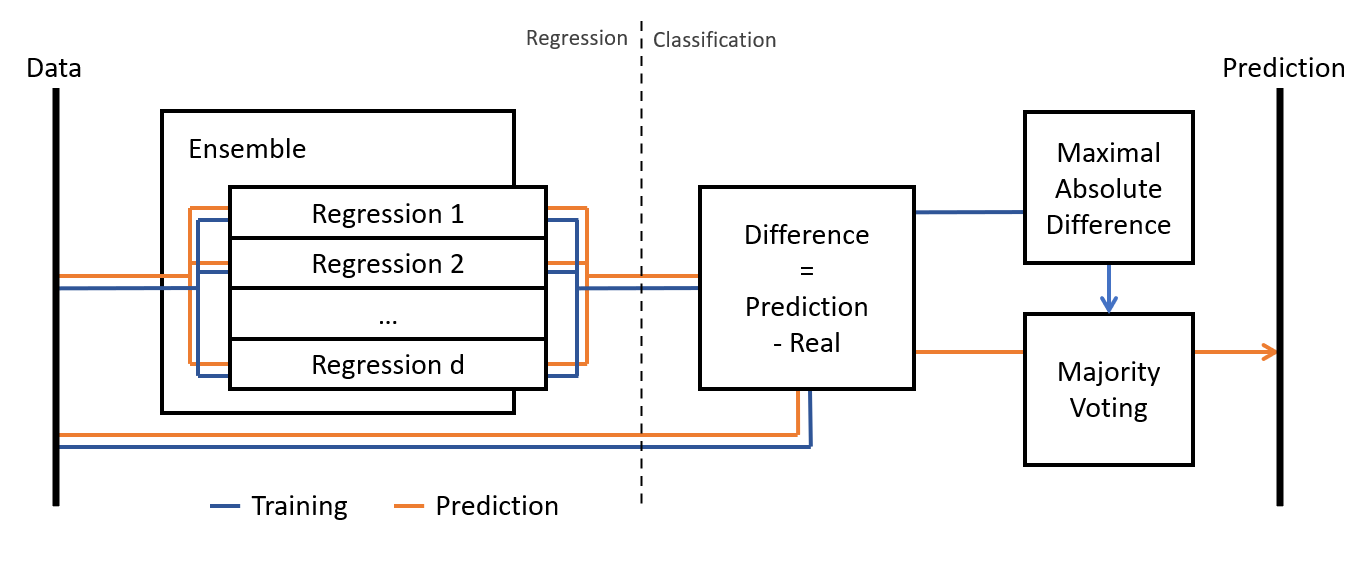
\includegraphics[width=0.9\textwidth]{res/practice-ensemble.png}}
    \caption{Schematische Darstellung des Regression-Ensemble-Ansatzes eingeteilt in die zwei Phasen.}
    \label{fig:practice-ensemble}
\end{figure}

Im Trainingsschritt werden die Listen an Zeitfolgen wie auch beim Klassifikationsansatz zuerst konkateniert.
 Diese Menge an Zeitpunkten wird nun in ein Ensemble an Regressionsalgorithmen geleitet. Dieses ist wie folgt
 aufgebaut:

\begin{itemize}
    \item Für jeden zu schätzenden Knoten gibt es genau einen Regressionsalgorithmus, welcher den Wert des Knoten
     schätzen soll.
    \item Welcher Algorithmus mit welcher Konfiguration der Hyperparameter dies ist, ist als Basemodel festgelegt.
    \item Die Eingabe jedes Basemodels sind die konkatenierten Daten mit jeweiliger Ausnahme der Werte des eigenen
     Knotens\footnote{Wichtig anzumerken ist hier, dass die Daten derart gefiltert werden, dass nur leckfreie
     Zeitpunkte für dieses Training genutzt werden. Im Kapitel \ref{Chapter-Discussion} wird dies weiter
     diskutiert.}.
\end{itemize}

Ist das Ensemble trainiert, wird es direkt benutzt um den digitalen Zwilling zu erschaffen. Die zweite Phase
 beginnt nun damit, die Differenzen zwischen realen und geschätzten Werten zu berechnen. Hierfür werden die
 geschätzten Werte einzeln von ihrem realen Gegenstück abgezogen. Es entsteht eine Differenzenmatrix
 $\mathcal{D} \in \mathbb{R}^{(N*p) \times d}$, die für leckfreie Zeitpunkte vom Betrag niedrige Werte und in
 Szenarien mit Leck hohe Werte haben soll. Um nun Thresholds zu berechnen wird für jeden Knoten die vom Betrag
 her maximale Differenz ausgewählt, welche einem leckfreien Zeitpunkt zugeordnet ist. Mit dem Hyperparameter
 \texttt{th\_multiplier} kann dieser noch um einen gewissen Prozentsatz vergrößert werden. Ein weiterer wichtiger
 Hyperparameter ist der \texttt{th\_mode}, welcher die Werte \texttt{simple} oder \texttt{daytime} annehmen kann.
 Der eben beschriebene Ablauf der Thresholdfindung ist die einfache Berechnung, während die Einstellung
 \texttt{daytime} die Differenzen zusätzlich nach der Tageszeit gruppiert. Während der Threshold-Vektor bei der
 einfachen Berechnung aus $\mathbb{R}^d$ ist, ist dieser nun aus $\mathbb{R}^{d \times tspd}$, wobei $tspd$ die
 Zeitschritte pro Tag angibt, also 24 bei dem ad-hoc Datensatz und 48 bei LeakDB.

Wie bei dem Klassifikationsansatz wird im Vorhersageschritt nun jede Zeitfolge einzeln betrachtet und dessen
 Ergebnisse nach Anwendung des Median-Filters in eine Ausgabeliste eingesetzt. Das Betrachten einer Zeitfolge
 sieht so aus, dass in der ersten Phase wieder mittels Regressions-Ensemble das geschätzte Netzwerk generiert
 und in der folgenden Phase mit den echten Werten zu einer Differenzenmatrix gemacht wird. Die im Trainingsschritt
 gefundenen Thresholds werden nun auf $\mathcal{D}$ angewendet. Dafür wird jeder Wert mit seinem Threshold,
 also nach Knoten und möglicherweise Tageszeit, verglichen. Ist der absolute Wert größer, so gibt der Knoten für
 den Zeitpunkt eine 1 aus, sonst würde er eine 0 ausgeben. Werden die Schätzungen der Knoten nun nach Zeitpunkt
 aufsummiert, erhält jeder Zeitpunkt die Anzahl der Knoten, die Alarm schlagen. Mit dem Hyperparameter
 \texttt{th\_majority} kann man einstellen, wieviel Prozent an Knoten warnen müssen, bevor der Zeitpunkt insgesamt
 als Leck gelabelt wird.

\section{Feature Extraction}

Ein weiteres Werkzeug zum Verbessern von Vorhersagen kann das Feature Extractions sein. Das ist eine Form des
 Preprocessings, bei dem die Daten transformiert werden um Features zu entfernen, modifizieren oder hinzuzufügen.
 Zwei in dieser Arbeit untersuchte Methoden werden im Folgenden vorgestellt.

\subsection*{Past Days Transform}

Die Past Days Transform versucht sich die annähernde Periodizität der Daten zu nutze zu machen, die bei
der Analyse der Daten herausgekommen ist. Dafür werden zu den Druckwerten an einem Zeitpunkt die jeweiligen
Druckwerte des letzten Tages hinzugefügt. Ein Datenpunkt sieht dann so aus:

\begin{equation*}
    x_{i, j} = (x_{i, j}^{(1)}, \dots, x_{i, j}^{(d)}, x_{i, j-tspd}^{(1)}, \dots, x_{i, j-tspd}^{(d)})
\end{equation*}

Dies kann rekursiv mehrere Male gemacht werden, wodurch ein Datenpunkt mehrere Tage in die Vergangenheit
 gucken kann. Der Parameter \texttt{past\_end} kontrolliert, wie viele Tage Rückblick betrachtet werden. Ist
 dieser beispielsweise auf Drei, so besitzt ein Datenpunkt die Druckwerte des eigenen Tages, des Tages
 zuvor und die des zwei Tage zurückliegenden Datums.

\subsection*{Mean Transform}

Um Rauschen entgegenzuwirken kann dass Mitteln der Werte in einem kleinen Fenster um die jeweiligen Werte helfen.
 Mean Transform implementiert genau diese Methoden. Dabei kann mit dem Parameter \texttt{window} die Größe des
 Fensters eingestellt werden.


\chapter{Ergebnisse}

Zum Generieren der Ergebnisse wurde Grid-Search auf beiden Datensätzen für beide Ansätze, Klassifikation und
 Regressions-Ensemble, angewendet. Da dabei alle möglichen Kombinationen der Hyperparameter getestet werden,
 kann man einerseits verhindern, in lokale Optima zu laufen, andererseits kostet dieses Verfahren eine lange
 Zeit. Damit ist sowohl die Generierung, als auch die Analyse gemeint, da die Anzahl an Ergebnissen durch das
 Produkt der jeweils möglichen Einstellungen der Hyperparameter gegeben ist. Existieren beispielsweise fünf
 Hyperparameter mit jeweils fünf Einstellungen, so ist die Anzahl an Durchläufen gleich $5^5=3125$.
 Eine Auflistung, wie viele Kombinationen getestet wurden, kann in Tabelle \ref{tab:res-kombs} eingesehen werden.

 \begin{table}[h]
    \centering
    \begin{tabular}{l|ll|ll}
    & \multicolumn{2}{l|}{Klassifikation} & \multicolumn{2}{l}{Regression-Ensemble} \\
    \hline
    Basemodel & \# HP & \# Kombi. & \# HP & \# Kombi. \\
    \hline
    LR        &                           &                                & \multicolumn{1}{c}{0}     & \multicolumn{1}{c}{300}       \\
    Ridge     &                           \multicolumn{2}{c|}{-}           & \multicolumn{1}{c}{1}     & \multicolumn{1}{c}{1800}      \\
    Lasso     &                           &                                & \multicolumn{1}{c}{1}     & \multicolumn{1}{c}{1800}      \\
    kNN       & \multicolumn{1}{c}{2}     & \multicolumn{1}{c|}{40}        & \multicolumn{1}{c}{2}     & \multicolumn{1}{c}{2400}      \\
    MLP       & \multicolumn{1}{c}{3}     & \multicolumn{1}{c|}{900}       & \multicolumn{1}{c}{3}     & \multicolumn{1}{c}{54000}
    \end{tabular}
    \caption{Anzahl (als \# abgekürzt) von Hyperparametern (HP) einzelner Modelle und ihrer insgesamter Anzahl an
        Kombinationen inklusive der Wrapper-Klasse. Klassifikation besitzt nur einen Hyperparameter, während
        Regression-Ensemble vier besitzt.}
    \label{tab:res-kombs}
\end{table}

Da eine detaillierte Analyse aller Kombinationen den Rahmen dieser Arbeit sprengen würde, werden für den
 Ad-Hoc Datensatz sowie für den Ansatz der Klassifikation bei dem LeakDB Datensatz nur die besten Konfigurationen
 präsentiert. Da der Regressions-Ensemble-Ansatz auf dem realistischeren Datensatz die wichtigsten Werte zeigt,
 wird dieser detaillierter betrachtet. Hier wird zuletzt auch die Detektionszeit und das Feature Extraction
 analysiert. Die vollständigen Werte jedes einzelnen Experimentes sind auf der GitHub-Seite als csv-Dateien
 bereitgestellt [TODO Quelle]. Dort ist ebenfalls ein Notebook namens \texttt{analyse.ipynb} hinterlegt, in welchem
 die komplette Analyse der Ergebnisse dokumentiert ist.

\section{Optimale Konfiguration}

Im Zuge des Ad-Hoc Datensatzes wurden 300 Zeitfolgen mit jeweiliger Zeitspanne von fünf Tagen getestet. Um die
 Accuracy als valide, erste Einschätzung der Güte nutzen zu können, ist der Datensatz genau zur Hälfte in
 leckfreie und leckbehaftete Szenarien aufgeteilt. Abbildung \ref{fig:res-best-adhoc} zeigt die Metriken der, nach
 Accuracy, besten Konfigurationen der jeweiligen Ansätze und Basemodels. Anhang \ref{appendix-best-conf} listet
 die jeweiligen Werte auf. Wichtig zu bemerken ist, dass k-Nearest Neighbors in beiden Ansätzen und allen Metriken
 den höchsten Wert von 100\% abliefert. Währenddessen sind bei der Linearen Regression und vor allem bei der
 L2-Regulierung starke Einbrüche in der Sensitivität für Lecks zu sehen.

Um auch bei LeakDB die Accuracy nutzen zu können, wurden aus den 1000 Szenarien 500 ausgewählt, sodass diese
 mit 250 leckfreien zu 250 leckbehafteten Szenarien balanziert war. Zusätzlich zu der doppelten, zeitlichen
 Auflösung, ist jede Zeitfolge hier zehn Tage lang. Abbildung \ref{fig:res-best-leakdb} zeigt wieder die besten
 Werte auf, dessen Konfigurationen in Anhang \ref{appendix-best-conf} wieder gezeigt werden. Hier ist zu bemerken,
 dass kNN aus dem Ansatz des Regressions-Ensembles stark eingebrochen ist, während die anderen Werte weitgehend
 stabil bleiben.

\begin{figure}[h]
    \centering
    \begin{subfigure}{\textwidth}
        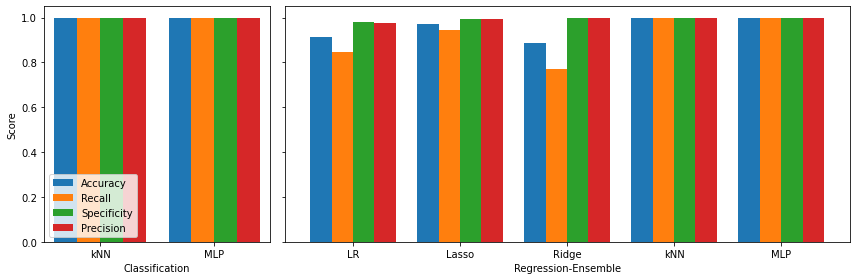
\includegraphics[width=1.0\textwidth]{res/res-best-adhoc}
        \caption{Ad-Hoc Datensatz\vspace{1em}}
        \label{fig:res-best-adhoc}
    \end{subfigure}
    \begin{subfigure}{\textwidth}
        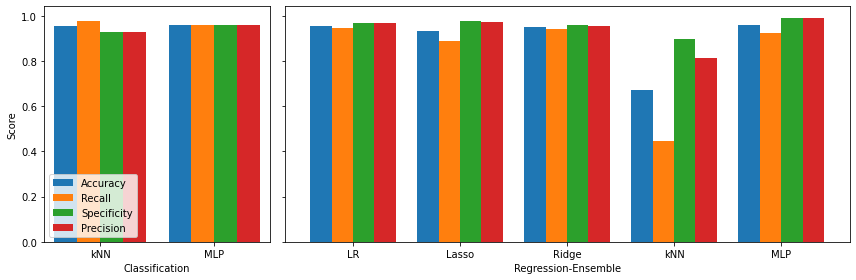
\includegraphics[width=1.0\textwidth]{res/res-best-leakdb}
        \caption{LeakDB}
        \label{fig:res-best-leakdb}
    \end{subfigure}
    \caption{Die Werte der besten Konfigurationen einzelner Modelle, nach der Akkuratheit.}
\end{figure}

\section{LeakDB Datensatz}

Um diese massiven Datenmengen analysieren zu können, wurde zuerst für jeden Hyperparameter ein Einfluss-Wert
 erzeugt. Dieser gibt Aufschluss darüber, wie viel Einfluss die Veränderung dieses Wertes auf das Ergebnis
 einer Metrik hat und wird wie folgt berechnet:

\begin{verbatim}
    def influence(results, feature, metric='accuracy'):
        grouped = results.groupby(feature).mean().loc[:, metric]
        return grouped.max() - grouped.min()
\end{verbatim}

Hierbei sind \texttt{results} die Ergebnisse aus der csv-Datei, \texttt{feature} das zu untersuchende Feature
 und \texttt{metric} die jeweilige Metrik. Die \texttt{groupby}-Funktion gruppiert also zuerst die Ergebnisse
 nach dem Hyperparameter, dessen Einfluss berechnet werden soll. Für jede seiner möglichen Einstellungen wird
 dann der mittlere Metrikwert berechnet, was dazu führt, dass die Differenz des maximalen zu dem minimalen
 Mittelwert den Gesamteinfluss widerspiegelt. Ein Hyperparameter mit einem Einfluss von 0.6 hat also das
 Potential, das Ergebnis um 0.6, also 60\%-Punkte, zu verändern, während ein Hyperparameter mit einem Einfluss
 von 0.01 nur wenig am Endergebnis verändern kann. Anhang \ref{appendix-ranking} gibt den Einfluss jedes
 möglichen Hyperparameters pro Basemodel an. Hier ist gut zu sehen, dass der Wrapper-spezifische Hyperparameter
 \texttt{th\_majority}, also die Anzahl, wie viele Knoten Alarm schlagen müssen, bevor ein Zeitpunkt als
 leckbehaftet gilt, tendenziell den größten Effekt auf das Endergebnis hat, während die Größe des Median-Filters
 nur einen sehr kleinen Effekt hat. Für kNN und MLP ist \texttt{th\_majority} jedoch nur an zweiter Stelle, da
 ihre modellspezifischen Hyperparameter \texttt{weights} und \texttt{activation} größeren Einfluss haben.

Die folgenden Analysen der Hyperparameter wurden generiert, indem die Hyperparameter mit höherem Einfluss auf
 ihre lokale Optima gesetzt wurden und die Werte der Hyperparameter geringerem Einflusses gemittelt wurden.
 So lassen sich Tendenzen in der Veränderung eines Hyperparameters isolierter betrachten. Alle Grafiken dieser
 Analyse sind im Anhang gezeigt, welche keine Korrelation ergibt.

Schaut man sich zuerst den verhältnismäßig einflussreichsten Hyperparameter \texttt{th\_majority} an, so fällt auf,
 dass der Verlauf bei allen Basemodels ungefähr gleich ist. Abbildung \ref{fig:res-th-majority} zeigt dies am
 Beispiel des MLPs. Während die Spezifität annähernd konstant bleibt, sinken die Werte der Sensitivität und
 Akkuratheit. Am interessantesten ist die Präzision, also der Anteil echter Lecks an den prognostizierten Lecks,
 welcher erst Nahe eins bleibt, dann aber plötzlich stark abfällt. Ein weiterer, einflussreicher
 Wrapper-Hyperparameter ist \texttt{th\_mode}, welche die Abhängigkeit der Thresholds von der Tageszeit einstellt.
 Auch hier sind die Verläufe ähnlich unter den Basemodels und liefert ein klares Bild: Die Thresholds von der
 Tageszeit abhängig zu machen verbessert die Akkuratheit und die Sensitivität, während die anderen Metriken sich
 nur leicht verschlechtern, wie am Beispiel der Linearen Regression in Abbildung \ref{fig:res-th-mode} zu sehen
 ist. Weniger Einfluss geht von \texttt{th\_multiplier} aus, welcher die berechneten Thresholds künstlich erhöhen
 kann. Abbildung \ref{fig:res-th-multiplier} zeigt die Interaktion mit \texttt{th\_majority} in einer Heatmap.

\begin{figure}
    \centering
    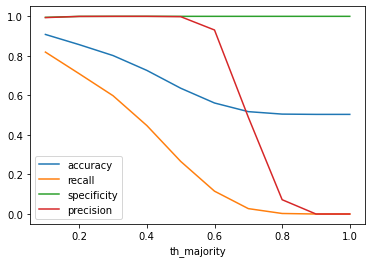
\includegraphics[width=0.7\textwidth]{res/res-th-majority}
    \caption{Durchschnittlicher Verlauf der Metriken für den Hyperparameter \texttt{th\_majority}.}
    \label{fig:res-th-majority}
\end{figure}

\begin{figure}
    \centering
    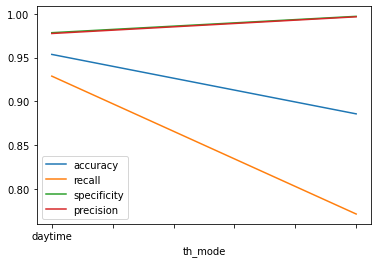
\includegraphics[width=0.7\textwidth]{res/res-th-mode}
    \caption{Durchschnittliche Werte der Metriken für \texttt{daytime} (links) und
        \texttt{simple} (rechts) des Hyperparameters \texttt{th\_mode}.}
    \label{fig:res-th-mode}
\end{figure}

\begin{figure}
    \centering
    \fbox{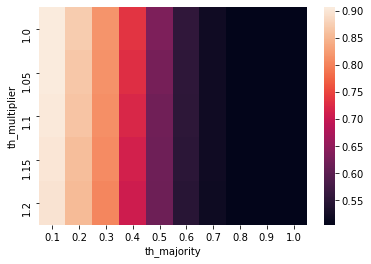
\includegraphics[width=0.7\textwidth]{res/res-th-multiplier}}
    \caption{2-dimensionaler Verlauf der Accuracy in Abhängigkeit der Hyperparameter \texttt{th\_multiplier} und
        \texttt{th\_majority} für die Ridge Regression.}
    \label{fig:res-th-multiplier}
\end{figure}

Für k-Nearest Neighbors ist der einflussreichste Hyperparameter \texttt{weights}, mit welchem angegeben werden
 kann, ob die Datenpunkte in der Nachbarschaft alle gleich gewichtet werden, oder nach ihrem Abstand. Der Effekt
 von distanzbasierter Gewichtung im Vergleich zur uniformen Gewichtung wird in Abbildung
 \ref{fig:res-knn-weights} gezeigt. Hier sieht man, dass die Spezifität abnimmt, während die Sensitivität
 erhöht wird. Bei der distanzbasierten Gewichtung werden also mehr Punkte als Leck klassifiziert.

\begin{figure}
    \centering
    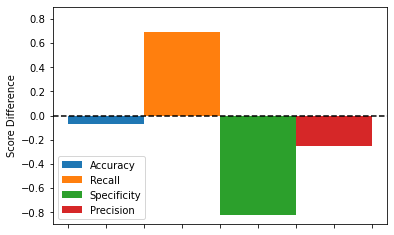
\includegraphics[width=0.7\textwidth]{res/res-knn-weights}
    \caption{Relative Veränderung der Metriken beim Umschalten auf distanzbasierten Gewichten für kNN.
        Sensitivität verbessert sich stark, während die Spezifität sich verschlechtert hat.}
    \label{fig:res-knn-weights}
\end{figure}

Betrachtet man das MLP, so ist die richtige Wahl der Aktivierungsfunktion am entscheidendsten. Abbildung
 \ref{fig:res-mlp-activation} zeigt, dass die Wahl der logistischen Funktion oder der Hyperbeltangens im
 Mittelwert zu einer Präzision und Sensitivität nahe null führt. Ein weiterer, nicht so einflussreicher
 Hyperparameter von MLP ist die Gestaltung der verborgenen Schichten. Auch, wenn es schwierig ist, eine Ordnung
 auf der Struktur zu finden, kann man in Abbildung \ref{fig:res-mlp-layers}, welche die Schichten zuerst nach
 ihrer Anzahl und dann ihrer Summe an Perzeptronen sortiert, einen kleinen Abwärtstrend in der Sensitivität
 sehen, je größer das künstliche, neuronale Netz ist.

\begin{figure}
    \centering
    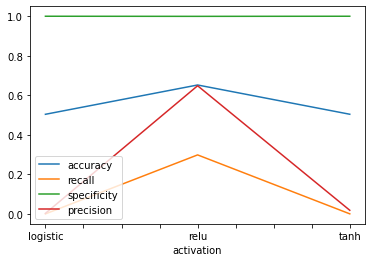
\includegraphics[width=0.7\textwidth]{res/res-mlp-activation}
    \caption{Durchschnittlicher Metrikwerte für die drei Aktivierungsfunktionen des MLPs.}
    \label{fig:res-mlp-activation}
\end{figure}

\begin{figure}
    \centering
    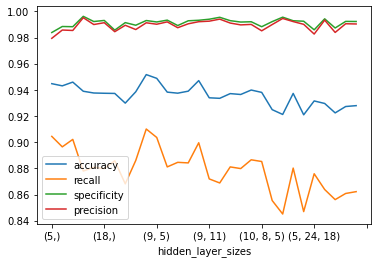
\includegraphics[width=0.7\textwidth]{res/res-mlp-layers}
    \caption{Durchschnittliche Metrikwerte abhängig von der Form der verborgenen Schichten.
        Dabei sind links tendenziell kleinere Netzwerke, während sie nach rechts wachsen.}
    \label{fig:res-mlp-layers}
\end{figure}


Für die meisten Hyperparameter ist das Optimum für die bisher betrachteten Metriken ebenso das der
 Detektionszeit. Ein davon abweichender Fall, welcher in Abbildung \ref{fig:res-fe-th-mode} gezeigt wird, ist der
 \texttt{th\_mode}, welcher im Gegensatz zu den anderen Metriken leicht die simple Einstellung bevorzugt.

\begin{figure}
    \centering
    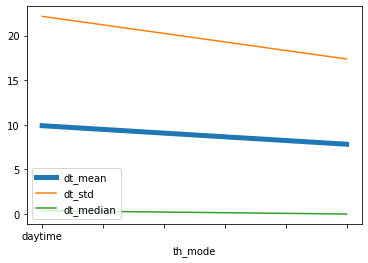
\includegraphics[width=0.7\textwidth]{res/res-fe-th-mode}
    \caption{Informationen über die Detektionszeit (dt) für \texttt{daytime} (links) und
        \texttt{simple} (rechts) des Hyperparameters \texttt{th\_mode} anhand Ridge.
        Dabei sind hier kleinere Werte besser, was \texttt{simple} etwas besser macht.}
    \label{fig:res-fe-th-mode}
\end{figure}

\section{Einfluss von Feature Extraction}

Um die Effekte der zwei Techniken der Feature Extraction zu analysieren wurde das Basemodel Ridge Regression
 für den Ansatz des Regression-Ensembles genutzt. Für die Past Days Transformation wurden Werte zwischen Eins,
 also keinem Rückblick, und Fünf, also ein Rückblick um bis zu vier Tage in die Vergangenheit, gewählt. Für
 die Mean Transformation wurde ebenso eine Fenstergröße von Eins, also keiner Veränderung, bis zu Fünf, also
 einer Mittelwertberechnung über fünf Werte, vorgegeben. Die Ergebnisse lassen sich als Heatmap in
 Abbildung \ref{fig:res-fe-metrics} einsehen. Interessant ist hier zu sehen, dass obwohl der Rückblick in die Vergangenheit generell
 bessere Werte liefert, so weiter dieser ist, ist für Accuracy und Sensitivity kein Rückblick am besten. Zudem
 kann die Mittelung der Werte nur bessere Werte hervorbringen, falls die Past Days Transform aktiv ist.

Betrachtet man sich jedoch die Detektionszeit in Abbildung \ref{fig:res-fe-dt}, so hat die Mittelung für die
 durchschnittliche Detektionszeit auch ohne Past Days Transform einen guten Effekt.

 \begin{figure}
    \centering
    \begin{adjustwidth}{-1cm}{}
        \begin{subfigure}{\textwidth}
            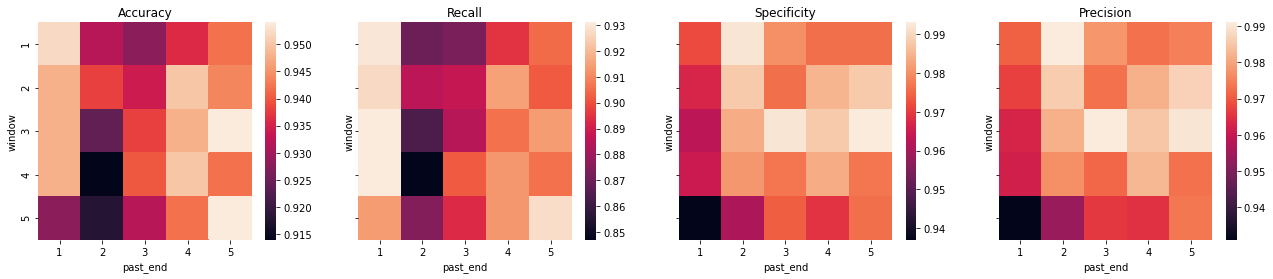
\includegraphics[width=1.3\textwidth]{res/res-fe-metrics}
            \caption{Die vier Metriken der Konfusionsmatrix.\vspace{1em}}
            \label{fig:res-fe-metrics}
        \end{subfigure}
        \begin{subfigure}{\textwidth}
            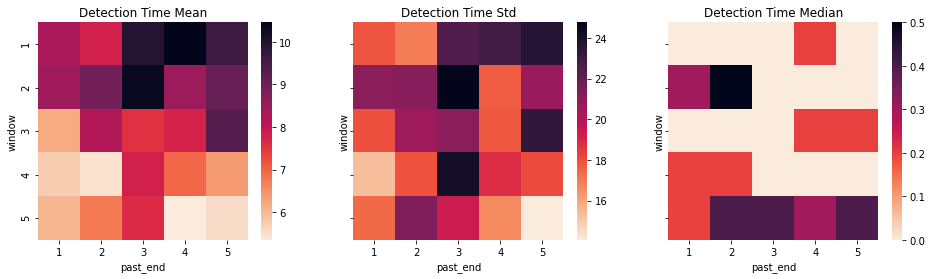
\includegraphics[width=0.9\textwidth]{res/res-fe-dt}
            \caption{Die Detektionszeit.}
            \label{fig:res-fe-dt}
        \end{subfigure}
        \caption{2-dimensionaler Verlauf durchschnittlicher Metrikwerte anhand der FE-spezifischen
            Hyperparameter \texttt{window} und \texttt{past\_end}. Hellere Werte sind hier besser.}
    \end{adjustwidth}
\end{figure}

\section{Diskussion \label{Chapter-Discussion}}

Um die Leistung verschiedener Ansätze des maschinellen Lernens in der Problemstellung der Leck-Detektion zu
 testen wurden diese zuerst auf einem einfachen und danach auf einem realistischeren Datensatz evaluiert. Dabei
 hat die Auswertung unter Anderem gezeigt, dass k-Nearest Neighbors sowohl im Ansatz der Klassifikation als auch
 des Regressions-Ensemble auf dem Ad-Hoc Datensatz beinahe perfekte Ergebnisse liefern kann, während es auf dem
 komplexen Datensatz stark schwächelt. Dies kann daran liegen, dass LeakDB neben den täglichen Schwankungen
 auch jährliche Veränderung besitzt, über die kNN keine Kenntnis haben kann. Die zusätzliche Angabe zum Beispiel
 der Kalenderwoche würde hier zwar vermutlich helfen, jedoch würde das viel mehr Daten erfordern. Zudem gibt es
 auch über Jahre hinweg andauernde Schwankungen durch das Weltklima, welche den Rahmen wieder sprengen würden.
 Die gegengesetzte Richtung, also dass Modelle auf den komplexeren Daten besser werden, ist bei den
 Regressionsalgorithmen zu sehen. Vor allem L2 kann hier signifikant an Sensitivität gewinnen. Ein möglicher
 Grund für die schlechtere Leistung auf den einfacheren Daten ist, dass diese anfangen, das Rauschen zu lernen,
 Stichwort Overfitting.

Ein weiterer großer Vorteil des Regression-Ensemble-Ansatzes ist, dass der Trainingsprozess nur leckfreie Daten
 benutzt. Das Modell kann also vollkommen auf leckbehaftete Zeitpunkte verzichtet, welche in manchen Städten rar
 sind.

Wichtig anzumerken ist jedoch, dass in der momentanen Implementation des Ensembles der Trainingsschritt noch
 ausgebessert werden kann. So werden aktuell auf allen (leckfreien) Datenpunkten trainiert und direkt
 prognostiziert, um die Differenzen, welche dann die Thresholds ergeben, zu berechnen. Das bedeutet, dass
 bereits gelernte Daten abgefragt werden, was, wie in Kapitel \ref{Chapter-ML} bereits gesagt, Probleme mit
 sich ziehen kann. Separates Training mit Cross Validation und extra Mengen alleine für die Berechnung der
 Differenzen kann zukünftig helfen, wobei ein solches Vorgehen wieder einen höheren Bedarf an Daten mit sich zieht.

Weitere Fragen, die sich aus der Analyse ergeben, sind die der einzelnen Hyperparameter. Betrachtet man
 \texttt{th\_majority}, so lässt sich das Absteigen von Sensitivität und Akkuratheit leicht erklären: Denn dieser
 Hyperparameter gibt die Anzahl an, wie viele Knoten Alarm schlagen müssen und erhöht damit die generelle Hürde,
 damit ein Zeitpunkt als Leck erklärt wird. Höhere Hürde trotz konstanter Werte führt zu geringeren Zahlen.
 Interessant ist jedoch die Präzision, welche zuerst stetig bei 100\% bleibt und dann plötzlich auf 0\%
 fällt. Aufschluss über dieses Verhalten gibt die Spezifität, welche hier bei 100\% liegt. Dieser Wert kann
 nur erreicht werden, wenn die Anzahl fälschlicherweise als positiv markierten Punkte (FP) gleich 0 ist.
 Für die Präzision, welche als $\frac{TP}{TP+FP}$ berechnet wird, bedeutet dies, dass sie nur die Werte 1, falls
 es mindestens ein richtigerweise positiv markierten Punkt gibt, oder 0, falls TP = 0 ist, erreichen
 kann\footnote{Bei TP = 0 würde die Formel zu $\frac{0}{0}$ evaluieren, was nicht definiert ist. Für diese Anwendung
 ist es jedoch als 0 definiert.}, was dieses Verhalten der Präzisionskurve erklärt. Die Werte zwischen 0 und 1
 stammen dabei aus der Mittelung der verschiedenen Konfigurationen. Bezüglich des Erhöhen der Hürde ist die
 Interaktion mit dem Hyperparameter \texttt{th\_multiplier} interessant. Da dessen Erhöhung ebenfalls eine
 Verstärkung der Hürde darstellt, könnte man meinen, dass diese Parameter in einer inversen Korrelation
 zueinander stehen sollten: So niedriger der Threshold, desto mehr Knoten sollte es zum Alarm schlagen
 benötigen. Doch die Abbildung \ref{fig:res-th-multiplier} unterstützt diese These nicht.

Betrachtet man die Aktivierungsfunktion des MLPs, so kann die gleiche Erklärung wie für den plötzlichen Abfall
 der Präzision bei \texttt{th\_majority} genutzt werden: Hier ist die Spezifität auch nahe 100\%, was für die
 logistische Funktion oder den Hyperbeltangens bedeutet, dass keine Zeitpunkte als Leck gelabelt wurden. Um
 den Einfluss der verborgenen Schichten eines MLPs genauer bestimmen zu können, muss dieser jedoch noch weiter
 getestet und analysiert werden. Für diese Tests wurde die Form zufällig gesampelt, das heißt, es wurden nicht
 alle Kombinationen ausgetestet. Vielleicht kann mit einer erschöpfenden Suche ein Besserer Zusammenhang
 gefunden werden.

Die Betrachtung der Detektionszeit zeigt keinen großen, von der der anderen Metriken abweichenden,
 Handlungsbedarf an. Der Unterschied in den gezeigten Beispielen betrifft meist nur unter zwei Zeitschritten,
 also bei LeakDB eine Stunde. Der maximale Median betrifft für die Evaluation des Feature Extraction nur einen
 halben Zeitschritt, was einer viertel Stunde entspricht.

Die größte Limitation betrifft jedoch das zugrunde liegende WDN. Denn mit nur neun Knotenpunkten ist das
 benutzte “Net1” ein sehr kleines Netzwerk, wodurch die Ergebnisse, selbst bei realistischer Simulation, ein
 verfälschtes Bild abgeben können. Weiterführend sollten die Modelle somit auf größeren Netzwerken getestet
 evaluiert werden.

Auch das Auffassen des Themas als Vorhersageproblem von Zeitfolgen kann in weiterer Forschung noch stärker
 exploriert werden, da die in dieser Arbeit betrachteten Algorithmen nur begrenzt zeitlichen Kontext inferieren
 können.



\chapter{Zusammenfassung}

\{TODO\}

\bibliographystyle{plain}
\bibliography{References.bib}

\appendix

\chapter{Anhang}

\section{Beste Konfigurationen \label{appendix-best-conf}}

\begin{table}[ht]
    \footnotesize
    \begin{tabular}{lllll}
    Ansatz              & Basemodel & Hyperparameter                & \multicolumn{2}{c}{Wert} \\ \hline
                        &           &                               & Ad-Hoc      & LeakDB      \\ \cline{4-5} 
    Klassifikation      & kNN       & \texttt{n\_neighbors}         & 3           & 7           \\
                        &           & \texttt{weights}              & uniform     & uniform     \\
                        &           & \texttt{mk\_size}             & 3           & 11          \\
                        & MLP       & \texttt{hidden\_layer\_sizes} & (18, 22)    & (22, 24, 6) \\
                        &           & \texttt{learning\_rate}       & constant    & constant    \\
                        &           & \texttt{activation}           & logistic    & relu        \\
                        &           & \texttt{mk\_size}             & 3           & 11          \\
    \end{tabular}
\end{table}
\begin{table}[ht!]
    \footnotesize
    \begin{tabular}{lllll}
    Ansatz              & Basemodel & Hyperparameter                & \multicolumn{2}{c}{Wert} \\ \hline
                        &           &                               & Ad-Hoc      & LeakDB      \\ \cline{4-5}
    Regression-Ensemble & LR        & \texttt{th\_mode}             & daytime     & daytime     \\
                        &           & \texttt{th\_multiplier}       & 1.0         & 1.0         \\
                        &           & \texttt{th\_majority}         & 0.1         & 0.1         \\
                        &           & \texttt{mk\_size}             & 3           & 3           \\
                        & Lasso     & \texttt{alpha}                & 1.998       & 0.333       \\
                        &           & \texttt{th\_mode}             & daytime     & daytime     \\
                        &           & \texttt{th\_multiplier}       & 1.0         & 1.0         \\
                        &           & \texttt{th\_majority}         & 0.1         & 0.1         \\
                        &           & \texttt{mk\_size}             & 3           & 3           \\
                        & Ridge     & \texttt{alpha}                & 0.333       & 0.333       \\
                        &           & \texttt{th\_mode}             & daytime     & daytime     \\
                        &           & \texttt{th\_multiplier}       & 1.0         & 1.0         \\
                        &           & \texttt{th\_majority}         & 0.1         & 0.1         \\
                        &           & \texttt{mk\_size}             & 3           & 3           \\
                        & kNN       & \texttt{n\_neighbors}         & 3           & 3           \\
                        &           & \texttt{weights}              & uniform     & uniform     \\
                        &           & \texttt{th\_mode}             & daytime     & daytime     \\
                        &           & \texttt{th\_multiplier}       & 1.15        & 1.2         \\
                        &           & \texttt{th\_majority}         & 0.1         & 0.2         \\
                        &           & \texttt{mk\_size}             & 7           & 3           \\
                        & MLP       & \texttt{hidden\_layer\_sizes} & (5, 12, 12) & (7, 6)      \\
                        &           & \texttt{learning\_rate}       & adaptive    & adaptive    \\
                        &           & \texttt{activation}           & logistic    & relu        \\
                        &           & \texttt{th\_mode}             & daytime     & daytime     \\
                        &           & \texttt{th\_multiplier}       & 1.0         & 1.1         \\
                        &           & \texttt{th\_majority}         & 0.1         & 0.1         \\
                        &           & \texttt{mk\_size}             & 3           & 3            \\
    \end{tabular}
\end{table}

\newpage
\phantom{phantom}
\newpage

\section{Einfluss der Hyperparameter \label{appendix-ranking}}

\begin{table}[ht]
    \footnotesize
    \begin{adjustwidth}{-3.5cm}{}
        \begin{tabular}{lllll}
        Basemodel & Accuracy                              & Sensitivity                           & Specificity                         & Precision                             \\ \hline
        LR        & \texttt{th\_majority (0.414)}         & \texttt{th\_majority (0.85)}          & \texttt{th\_majority (0.012)}       & \texttt{th\_majority (1.0)}           \\
                  & \texttt{th\_mode (0.054)}             & \texttt{th\_mode (0.111)}             & \texttt{th\_mode (0.002)}           & \texttt{th\_mode (0.025)}             \\
                  & \texttt{th\_multiplier (0.01)}        & \texttt{th\_multiplier (0.021)}       & \texttt{th\_multiplier (0.001)}     & \texttt{mk\_size (0.01)}              \\
                  & \texttt{mk\_size (0.004)}             & \texttt{mk\_size (0.008)}             & \texttt{mk\_size (0.0)}             & \texttt{th\_multiplier (0.001)}       \\
        Lasso     & \texttt{th\_majority (0.338)}         & \texttt{th\_majority (0.7)}           & \texttt{th\_majority (0.011)}       & \texttt{th\_majority (1.0)}           \\
                  & \texttt{th\_mode (0.021)}             & \texttt{th\_mode (0.044)}             & \texttt{th\_multiplier (0.001)}     & \texttt{th\_multiplier (0.001)}       \\
                  & \texttt{alpha (0.012)}                & \texttt{alpha (0.025)}                & \texttt{th\_mode (0.001)}           & \texttt{th\_mode (0.001)}             \\
                  & \texttt{th\_multiplier (0.008)}       & \texttt{th\_multiplier (0.017)}       & \texttt{alpha (0.001)}              & \texttt{alpha (0.001)}                \\
                  & \texttt{mk\_size (0.005)}             & \texttt{mk\_size (0.011)}             & \texttt{mk\_size (0.0)}             & \texttt{mk\_size (0.0)}               \\
        Ridge     & \texttt{th\_majority (0.398)}         & \texttt{th\_majority (0.829)}         & \texttt{th\_majority (0.022)}       & \texttt{th\_majority (1.0)}           \\
                  & \texttt{th\_mode (0.054)}             & \texttt{th\_mode (0.112)}             & \texttt{th\_multiplier (0.002)}     & \texttt{th\_multiplier (0.002)}       \\
                  & \texttt{th\_multiplier (0.009)}       & \texttt{th\_multiplier (0.021)}       & \texttt{th\_mode (0.002)}           & \texttt{th\_mode (0.002)}             \\
                  & \texttt{mk\_size (0.007)}             & \texttt{mk\_size (0.014)}             & \texttt{mk\_size (0.0)}             & \texttt{mk\_size (0.0)}               \\
                  & \texttt{alpha (0.0)}                  & \texttt{alpha (0.0)}                  & \texttt{alpha (0.0)}                & \texttt{alpha (0.0)}                  \\
        kNN       & \texttt{weights (0.066)}              & \texttt{weights (0.693)}              & \texttt{weights (0.82)}             & \texttt{th\_majority (0.309)}         \\
                  & \texttt{th\_majority (0.058)}         & \texttt{th\_majority (0.451)}         & \texttt{th\_majority (0.332)}       & \texttt{weights (0.252)}              \\
                  & \texttt{th\_mode (0.012)}             & \texttt{mk\_size (0.065)}             & \texttt{mk\_size (0.059)}           & \texttt{n\_neighbors (0.017)}         \\
                  & \texttt{n\_neighbors (0.009)}         & \texttt{th\_mode (0.042)}             & \texttt{th\_mode (0.018)}           & \texttt{th\_mode (0.016)}             \\
                  & \texttt{mk\_size (0.002)}             & \texttt{n\_neighbors (0.035)}         & \texttt{n\_neighbors (0.017)}       & \texttt{th\_multiplier (0.007)}       \\
                  & \texttt{th\_multiplier (0.001)}       & \texttt{th\_multiplier (0.008)}       & \texttt{th\_multiplier (0.006)}     & \texttt{mk\_size (0.004)}             \\
        MLP       & \texttt{activation (0.148)}           & \texttt{activation (0.299)}           & \texttt{th\_majority (0.002)}       & \texttt{activation (0.645)}           \\
                  & \texttt{th\_majority (0.136)}         & \texttt{th\_majority (0.275)}         & \texttt{activation (0.001)}         & \texttt{th\_majority (0.393)}         \\
                  & \texttt{th\_mode (0.011)}             & \texttt{th\_mode (0.022)}             & \texttt{th\_multiplier (0.0)}       & \texttt{hidden\_layer\_sizes (0.029)} \\
                  & \texttt{hidden\_layer\_sizes (0.009)} & \texttt{hidden\_layer\_sizes (0.019)} & \texttt{th\_mode (0.0)}             & \texttt{th\_mode (0.017)}             \\
                  & \texttt{th\_multiplier (0.004)}       & \texttt{th\_multiplier (0.008)}       & \texttt{mk\_size (0.0)}             & \texttt{th\_multiplier (0.007)}       \\
                  & \texttt{mk\_size (0.002)}             & \texttt{mk\_size (0.003)}             & \texttt{learning\_rate (0.0)}       & \texttt{mk\_size (0.003)}             \\
                  & \texttt{learning\_rate (0.0)}         & \texttt{learning\_rate (0.0)}         & \texttt{hidden\_layer\_sizes (0.0)} & \texttt{learning\_rate (0.003)}      
        \end{tabular}
        \caption{todo: caption nur auf regr leakdb}
    \end{adjustwidth}
\end{table}



\end{document}